$K$-Nearest Neighbours ($K$NN), as the name suggests, is the process of finding $K$ nearest neighbours to a given query point. In this project, $K$NN query is only performed on $2$-dimensional data. We use $\ell_2$ norm as the distance metric. A $K$NN query will be formalised as $\mathcal{K}(\boldsymbol{X})$ where $\boldsymbol{X}\in\mathbb{R}^2$.

\subsubsection{$K$NN query with $K$D-Tree}
As a baseline, we first perform $K$NN query with $K$D-tree.\\
The main advantage of $K$D-Tree is that we can exploit the tree structure and prune points we don't think will have distance smaller than the ones we have already calculated. This improves the time complexity as compared to finding the distance of point with every other point in space to get the closest neighbours. 


\begin{algorithm}[H]
    \SetAlgoLined
    \SetKwInOut{Input}{Input}
    \SetKwInOut{Output}{Output}
    \Input{$K$; \texttt{Number of nearest neighbour, List of TestPoints; $\mathcal{P}(\boldsymbol{x}, \boldsymbol{y}); [x \in \mathbb{R};y \in \mathbb{R}]$}}
    \Output{\texttt{List of $K$ nearest points(ResultList)}}
    \For{$i\gets0$ \KwTo $len(TestPoints)$}
    {
        \texttt{Start at root}\\
        \texttt{Traverse subtree where $\mathcal{P}(\boldsymbol{x}, \boldsymbol{y})_i$ can be added.}\\
        \texttt{Find the leaf; Calculate the distance and store it as $\mathcal{D}$}\\
        \eIf{$len(ResultList) < K$}
            {
                \eIf {\texttt{Perpendicular distance of Parent with $\mathcal{P}(\boldsymbol{x}, \boldsymbol{y}) <= \mathcal{D}$}}
                    {
                        \texttt{Go on the other side of subtree} 
                    }
                        {
                            \texttt{Go up another $level$}
                        }
            }
            {
                \texttt{return ResultList}
            }
        
    }
    \caption{$K$NN Query Algorithm for $K$D-Tree}
    \label{$K$NN_Query_Algorithm_$K$D-Tree}
\end{algorithm}

In algorithm \ref{$K$NN_Query_Algorithm_$K$D-Tree},
\begin{enumerate}
    \item Start with the root to traverse tree until we reach the leaf. We find the subtree where the new $\mathcal{P}(\boldsymbol{x}, \boldsymbol{y})$ could be added and finally reach the leaf of this subtree. 

    \item Calculate the square of the euclidean distance of this point from the $\mathcal{P}(\boldsymbol{x}, \boldsymbol{y})$. We add it to the list and push and pop values from the list depending on the distances we calculate while traversing the tree upwards from here.
    
    \item From the leaf we could either go up another level or go the other side of the subtree to get a point that could have a distance smaller than the last best calculated distance in the list. 
    
    \item Once we make a decision in the above step, we can recursively traverse the tree upwards until we reach the root. 
\end{enumerate}


\begin{mscexample}


    \begin{minipage}[t]{\linewidth}
        \centering
        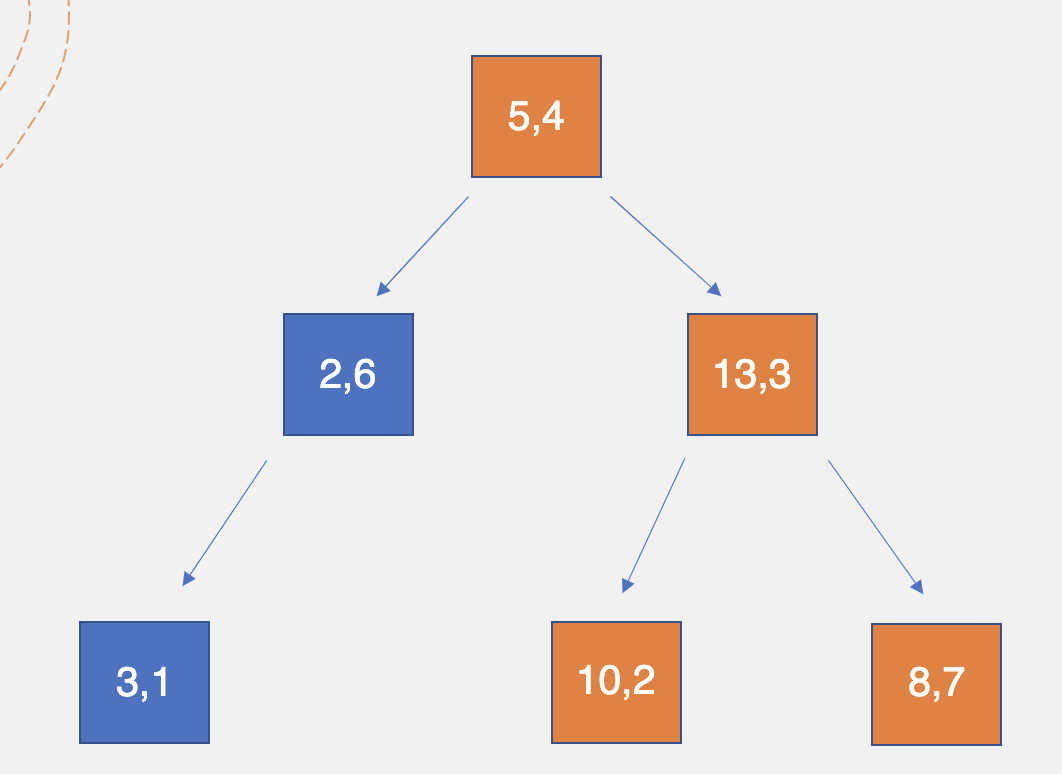
\includegraphics[width=6cm]{graphs/KD-Tree_KNN_Tree.png}
        % \caption{$K$D-Tree for KNN Query}
        \label{fig:$K$D-Tree_for_KNN Query}
        \hfill
        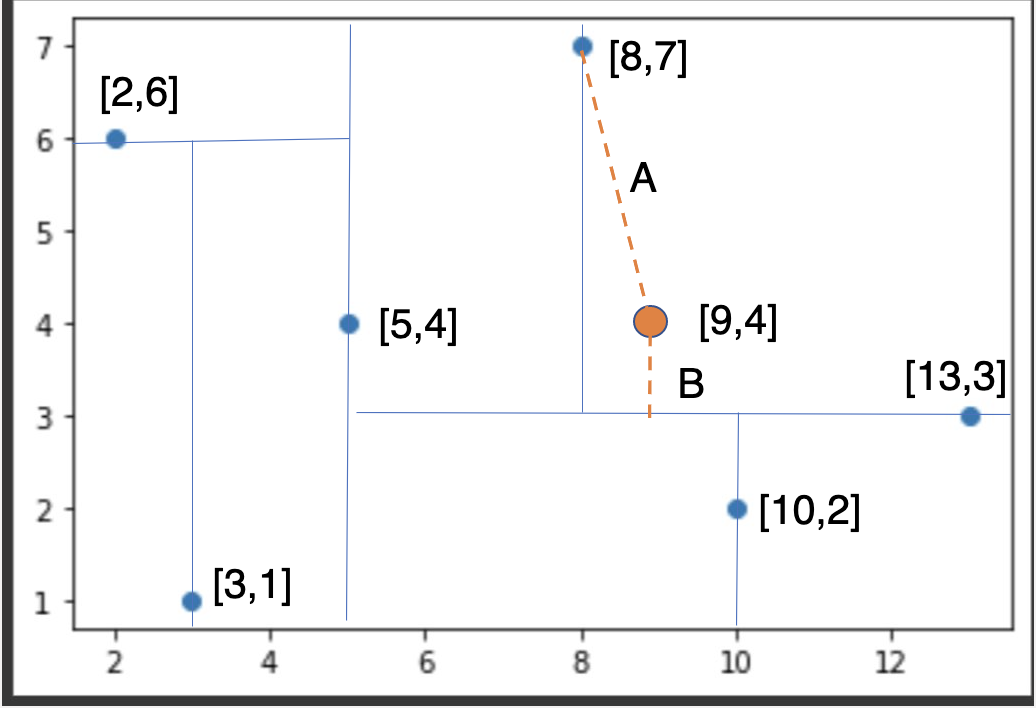
\includegraphics[width=6cm]{graphs/KD-Tree_KNN_plot.png}
        % \caption{$K$D-Tree KNN Plot on 2-dimentional plane}
        \label{fig:KD_Tree_KNN_Plot}
    \end{minipage}
	For example, we have Point list as $$((5,4),(2,6),(13,3),(8,7),(3,1),(10,2))]$$ 
	
	\textbf{Test point; $\mathcal{P}(\boldsymbol{x}, \boldsymbol{y})$} = $(9,4)$\\
	
% 	we will have a tree structure as shown in \ref{fig:$K$D-Tree_for_KNN Query} and it's plot on $2$-dimensional plane is shown in \ref{fig:KD_Tree_KNN_Plot}. *****\ref{fig:KD_Tree_KNN_Plot} \\
% 	In the fig above, we can see that although point $(8,7)$ is the leaf we will reach when we traverse the tree to search where test point $(9,4)$ can be added, it is not in fact the nearest point to the test point. \\
	
	Below are the steps followed to get the $4$ nearest neighbours:
	\begin{enumerate}
    	\item Traverse to $(8,7)$ by searching for a location where $\mathcal{P}(\boldsymbol{x}, \boldsymbol{y})$ could be added.
    	
    	\item Add $(8,7)$ to result list.
    	
    	\item Calculate the distance of $(8,7)$ and $\mathcal{P}(\boldsymbol{x}, \boldsymbol{y})$. Save the distance as $\mathcal{D}$
    	
    	\item Make a decision whether to traverse to the other side of the subtree to point $(10,2)$ by checking the perpendicular distance of $(13,3)$ with $\mathcal{P}(\boldsymbol{x}, \boldsymbol{y})$ and compare this with $\mathcal{D}$.(We do this to verify if there is even a possibility to find a point smaller than the last best distance on the other side of the subtree.) 
    	
    	\item Since the perpendicular distance is smaller than the best calculated $\mathcal{D}$ ($A > B$), we will check the distance of $\mathcal{P}(\boldsymbol{x}, \boldsymbol{y})$ and $(10,2)$. This distance in our case is indeed smaller than the best calculated distance of $\mathcal{P}(\boldsymbol{x}, \boldsymbol{y})$ with $(8,7)$ so far.
    	
    	\item Add $(10,2)$ to result list.
    	
    	\item Similarly, we traverse until we have $4$ nearest neighbour to $\mathcal{P}(\boldsymbol{x}, \boldsymbol{y})$ in the list.
	\end{enumerate}
\end{mscexample}



\subsubsection{$K$NN Query with LISA}
%TODO: What does this paragraph mean?
%We do not know the analytical representation of shards, as we use machine learning model $ \mathcal{SP}$ to generate shards. Thus, 
It is difficult to apply traditional $K$NN query pruning strategies applicable for $K$D-Trees, to LISA model as it doesn't maintain a tree like structure with all nodes and
entries based on MBRs (minimum bounding rectangle) and parent-children relationships. Shard boundaries are learned per mapped interval and no data structure is maintained to refer to shards in adjacent mapped intervals. The key idea in the $K$NN query is to convert it into a range query by estimating an appropriate query range. LISA paper suggests a learning model to learn an appropriate distance bound from underlying training data for every query point and specific value of K. However, we used empirically estimates to learn this distance bound for different values of $K$. This distance bound is used to convert the $K$NN query to range query.The query range is augmented if less than K neighbors are found in a range query. 

Consider a query point $q_{knn}=(x_{0},x_{1})$, let $x^{'} \in V$ be the $K$th nearest key to $x$ in database at a distance value $\delta = \| x^{'}-q_{knn}\|_{2} $. Lets define $ \mathcal{Q}(q_{knn},\delta) \triangleq [x_{0}-\delta, x_{0}+\delta) \times[x_{1}-\delta, x_{1}+\delta)$ and $\mathcal{B}(q_{knn}, \delta)  \triangleq \{p \in V \mid \| q_{knn}-p\|_{2} \leq \delta \} $. We can create a query rectangle $qr =  \mathcal{Q}(q_{knn}, \delta + \epsilon)$ where $\epsilon \rightarrow 0$. As shown in Fig. \ref{fig:KNN_Query_Lisa}, K nearest keys to $q_{knn}$ are all in $\mathcal{B}(q_{knn}, \delta)$ and thus in $\mathcal{Q}$. $K$NN query can be solved using the range query if we can estimate an appropriate distance bound $\delta$ for every query point.

\begin{figure*}[t]
    \centering
    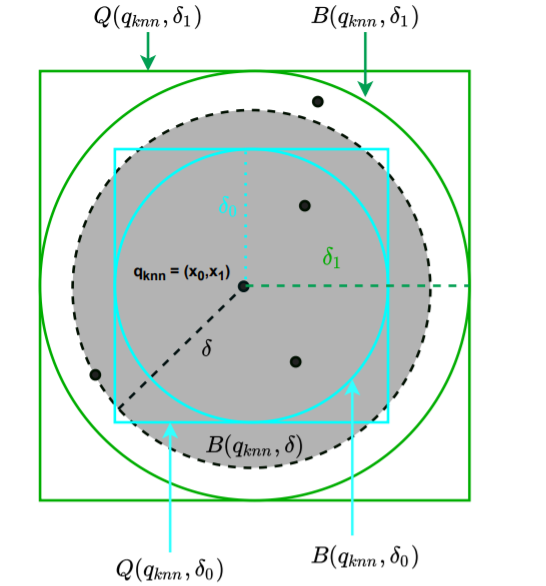
\includegraphics[width=0.7\textwidth]{graphs/KNN_Query_Lisa.png}
    \caption{KNN Query Implementation in Lisa(K=3)\\
    1)$q_{knn}$ represents the query point, $ \mathcal{Q}(x,\delta) \triangleq [x_{0}-\delta, x_{0}+\delta) \times[x_{1}-\delta, x_{1}+\delta)$, represents query rectangle and $ \mathcal{B}(x, \delta)$ represents the key space at distance $\delta$ containing K nearest keys.\\
    2)KNN query can be solved by range query if we can estimate an appropriate distance bound $\delta$ for every query point\\
    }
    \label{fig:KNN_Query_Lisa}
\end{figure*}
In our experiments, we find the $\delta$ empirically. We try with different values of $\delta$ and choose the one for which we get the best results. 